\documentclass[conference,letterpaper,10pt]{IEEEtran}
\usepackage{fontspec}
\setmainfont{Times New Roman}
\usepackage{amsmath,graphicx,booktabs,cite,url,balance}
\usepackage[hidelinks]{hyperref}
\hypersetup{pdftitle={Vigilant: LLM and RAG-Enhanced Agentic Framework for Continuous Software Traceability and Consistency Assurance across Requirements, Code, and Tests},pdfauthor={Ankith Singh}}
\begin{document}
\title{Vigilant: LLM and RAG-Enhanced Agentic Framework for Continuous Software Traceability and Consistency Assurance across Requirements, Code, and Tests}
\author{\IEEEauthorblockN{Ankith Singh}}
\maketitle
\begin{abstract}
Software changes can invalidate relationships among requirements, implementations, and tests even when individual artifacts remain syntactically valid. Trace-link recovery alone does not establish that related artifacts remain consistent. Vigilant combines versioned artifact extraction, a structural knowledge graph, hybrid retrieval, and a bounded agent workflow to assemble verifiable evidence for change investigations. A local Qwen2.5-1.5B-Instruct model produces constrained decisions, while deterministic rules and model judgments remain separately recorded. We evaluate trace-link ranking on SMOS, iTrust, English eTour, and a module-level RTMX subset, totaling 251 linked queries, and examine 12 authored change scenarios through 60 model calls. Compared with hybrid retrieval, RAG reranking changes mean average precision from 0.3026 to 0.3061 on SMOS and from 0.4406 to 0.4427 on eTour, but reduces it on iTrust and RTMX. All consistency variants return uncertain decisions, yielding 25\% agreement with authored labels, equal to an always-uncertain baseline. A recorded repository investigation verifies 24 evidence excerpts but does not establish semantic correctness. The contribution is an auditable implementation and a scoped empirical assessment that separates retrieval performance, evidence validity, and consistency assurance rather than treating them as interchangeable outcomes.
\end{abstract}
\begin{IEEEkeywords}
software traceability, requirements engineering, retrieval-augmented generation, knowledge graphs, large language models, change impact analysis, agentic workflows
\end{IEEEkeywords}
\section{Introduction}
Requirements, source code, and tests evolve at different rates. An endpoint can change while a client retains its former route; a requirement can be revised without corresponding implementation changes; or a test can disappear while the functionality it checked remains. Developers need both traceability, which identifies relationships between artifacts, and consistency assessment, which asks whether those related artifacts still agree at a particular revision. A plausible trace link is therefore useful evidence, but does not prove conformance.

Automated traceability research spans lexical retrieval, learned representations, and language models \cite{slr}. Lexical methods are inexpensive and reproducible but depend on shared vocabulary. Semantic representations can bridge terminology differences while also retrieving topically similar, functionally unrelated code. Static relations expose repository structure, yet cannot alone establish that a behavior satisfies a natural-language requirement. Retrieval-augmented generation (RAG) supplies external evidence to a generator \cite{rag}; traceability-specific work such as LiSSA already applies this principle across artifact types \cite{lissa}. The practical issue addressed here is how to combine retrieval with revision-specific evidence and bounded investigation without presenting generated explanations as verified software behavior.

Vigilant implements a repository analysis workflow in which artifacts, graph relationships, retrieved excerpts, rule findings, and model outputs retain distinct identities and provenance. Its agent roles execute a prescribed sequence of tools; they do not form an autonomous population of independently reasoning models. Similarly, ``continuous'' denotes the implemented ability to trigger analysis on repository changes, not an experimentally established guarantee of continuous correctness.

This paper contributes: (1) an implemented, version-aware architecture connecting requirements, code, tests, structural graphs, and checked excerpts; (2) a comparison of lexical, semantic, hybrid, graph-assisted, and local-LLM reranking methods across four scoped datasets; and (3) a controlled consistency study and recorded end-to-end investigation that expose the gap between retrieving valid evidence and making correct consistency judgments. The evaluation reports mixed and negative results rather than claiming a universally superior model.

\section{Related Work}
\textit{Retrieval and learned traceability.} The review by Alturayeif \emph{et al.} organizes machine-learning approaches to software traceability \cite{slr}. BM25 provides a lexical ranking basis \cite{bm25}, whereas Sentence-BERT provides a framework for sentence embeddings suitable for similarity retrieval \cite{sbert}. These methods motivate complementary baselines rather than an assumption that dense representations dominate lexical matching. Vigilant uses a pretrained MiniLM encoder and retains per-project comparisons to expose differences in vocabulary and link density.

\textit{RAG and LLM filtering.} LiSSA investigates generic RAG-based link recovery across several artifact relationships \cite{lissa}. Hey \emph{et al.} study RAG for inter-requirements traceability \cite{reqrag}; that task should not be conflated with requirement-to-code retrieval. Fuch\ss{} \emph{et al.} examine LLM ensembles for candidate filtering \cite{ensemble}. These studies motivate separating candidate retrieval from model-based acceptance. Our local reranker reviews only five candidates and preserves the candidate set, making its effects on ranking distinguishable from recall improvements that would require broader retrieval. We do not compare our scores directly with published scores produced under other protocols.

\textit{Structure, consistency, and agents.} Keim \emph{et al.} use recovered links to detect inconsistencies in architecture documentation \cite{archcons}; TransArC connects documentation and code through intermediate architecture information \cite{transarc}. Vigilant instead records source-level dependencies and revision changes to gather review evidence across requirements, code, and tests. Structural connectivity remains a candidate impact relation, not proof of propagation. SWE-agent illustrates the role of agent--computer interfaces in software engineering tasks \cite{sweagent}; Vigilant's prescribed tool sequence is substantially more restricted. Its contribution lies in integrating change provenance, evidence verification, and explicit uncertainty within this bounded workflow, with an evaluation that keeps retrieval and consistency outcomes separate.

\section{Proposed Methodology and System Architecture}
\subsection{Versioned Artifacts and Structural Graph}
The implementation uses a Python/FastAPI backend, SQLAlchemy persistence with SQLite, and a React interface. Git base and head revisions supply repository snapshots. Python AST parsing and Tree-sitter parsers for Java, JavaScript, and TypeScript extract supported source artifacts; requirement text, tests, and literal API declarations or client calls provide additional evidence. Imported repository code is parsed, not executed. Unsupported constructs and dynamic dispatch limit extraction completeness.

Each canonical artifact records project, repository, path, type, symbol, revision, and content hash. Identity and content version are separate: a stable symbol can change content between commits. NetworkX represents a directed multigraph whose persisted relationships include calls, imports, tests, API exposure and consumption, dependencies, and commit modifications. Static name matching and literal routes support these edges; they are not a whole-program semantic analysis. Recovered similarity links retain candidate status instead of becoming trusted implementation relationships.

Figure~\ref{fig:architecture} shows the investigation data flow. Base and head graphs are composed for impact exploration. The implementation traverses an undirected view for at most two hops, excluding default reverse-containment expansion. This identifies nearby candidates in either revision, including relationships lost after a change. It can also over-approximate impact, so graph reachability is never reported as a confirmed defect.
\begin{figure}[t]
\centering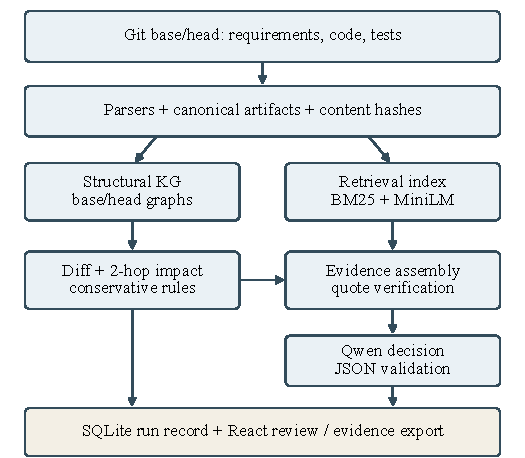
\includegraphics[width=\columnwidth]{figures/architecture.pdf}
\caption{Implemented investigation architecture. A prescribed workflow orchestrates these components. Rule findings and model decisions are persisted separately; graph edges and retrieved links remain evidence candidates.}
\label{fig:architecture}
\end{figure}

\subsection{Retrieval and Evidence Assembly}
Lexical retrieval uses normalized tokens, including split identifiers, with TF-IDF or BM25. Dense retrieval uses \texttt{all-MiniLM-L6-v2}, producing 384-dimensional vectors \cite{minilm}. Target text is divided into chunks of 180 normalized words, with at most eight chunks. Chunk vectors are averaged and normalized. The cap can omit late content in long files. Embeddings use CPU float32, batch size 24, and four threads, with a text-and-model-keyed SQLite cache.

Hybrid retrieval applies reciprocal rank fusion (RRF) \cite{rrf}:
\begin{equation}
 S(q,d)=\frac{1}{60+r_B(q,d)}+\frac{1}{60+r_E(q,d)},
\end{equation}
where $r_B$ and $r_E$ are one-based BM25 and embedding ranks of target $d$ for query $q$. The graph baseline combines $0.85$ times normalized hybrid relevance with $0.15$ times mean neighboring relevance from extracted file-level call, import, and test edges. Isolated targets retain their own relevance as the neighborhood term. Gold trace links are not used as graph edges. These exploratory weights are fixed for the reported run, not established optimal parameters.

Two RAG paths must be distinguished. The investigation path combines retrieved and graph-selected artifacts, changed seeds, and available before/after evidence. Retrieval and graph selection each use a depth of eight; an initial 8,000-character budget collects excerpts of up to 24 lines, with additional targeted temporal and rule evidence. Thus, the initial budget is not a strict bound on the final assembled packet. Each excerpt is checked against its source revision, path, lines, and hash. The measured investigation prompt then selects only the first six excerpts and at most 400 characters from each; the question is limited to 1,200 characters. Checked evidence in the report can therefore exceed what the model actually sees.

The traceability experiment instead presents a requirement prefix of at most 900 characters and five candidate prefixes of at most 1,100 characters each. Qwen labels candidates \texttt{SUPPORTED}, \texttt{UNSUPPORTED}, or \texttt{UNCERTAIN} using evidence aliases. Only supported candidates are promoted within the original top five; all others preserve hybrid order. Membership of the top five and top ten cannot change. Consequently, any measured benefit concerns ranking within a fixed candidate set.

\subsection{LLM, Agent Workflow, and Decisions}
The measured generator is \texttt{Qwen2.5-1.5B-Instruct} \cite{qwen}, executed locally on CPU in bfloat16 with four threads. Decoding is greedy, inputs exceeding 3,072 tokens are rejected, output at 220 new tokens, and a grammar constrains JSON generation. Neither the generator nor encoder is fine-tuned. Strict validation checks decision fields, statuses, cited aliases, and affected-artifact identifiers. Invalid responses are retained with an uncertain outcome. Valid JSON or a valid source quote does not establish that the model's interpretation follows from that quote.

The bounded orchestration has 12 stages: resolve revisions; import snapshots; compute differences; build base and head graphs; collect impact candidates; recover trace candidates; retrieve evidence; apply rules; verify excerpts; request the model decision; and persist the run. Role labels organize responsibilities within this sequence, but the model does not independently choose tools or iterate until a claim is proven. Conservative rules flag, for example, a removed endpoint, a changed implementation with unchanged tests, a deleted last-known test, or an obsolete client route. Findings are review hypotheses with source evidence. The final record separately stores rule findings, model status, confidence, uncertainty, citations, and execution outcomes. Completing every tool stage does not imply that the model has resolved the investigation.

A repository watcher can trigger analysis when Git HEAD changes. The implementation uses in-process execution and SQLite rather than a durable distributed job queue. An OmniRoute adapter was subsequently implemented, but no live gateway evaluation is included; every reported LLM result below comes from the pinned local Qwen model.

\section{Experimental Setup}
\subsection{Research Questions and Data}
The evaluation asks: RQ1, how do ranking methods compare under the same linked-query policy? RQ2, do additional evidence and bounded investigation improve consistency judgments on controlled changes? RQ3, can a complete change investigation retain checked evidence and distinguish execution success from model certainty?

Table~\ref{tab:setup} summarizes the retrieval datasets and configuration. SMOS, iTrust, and English eTour originate from the LiSSA replication package, pinned to commit \texttt{a8e652f29bbd}; RTMX \cite{rtmx} is pinned to \texttt{c2ced5349577}. Full commit hashes and model revisions accompany the reproduction materials. The three Java datasets serve as training, validation, and test projects for the optional learned ranker, respectively; the nonlearned baselines share the same prepared targets and queries. RTMX is an external, module-level subset, not a function-level benchmark. Two missing modules and unresolved function-level annotations preclude interpreting its 22 retained queries as the original broader task.
\begin{table}[t]
\caption{Datasets and principal experimental settings}
\label{tab:setup}\centering
\begin{tabular}{@{}lrrrr@{}}\toprule
Dataset / role & Req. & Linked & Targets & Links\\\midrule
SMOS / train & 67 & 67 & 100 & 1,044\\
iTrust / validation & 131 & 105 & 226 & 286\\
eTour English / test & 58 & 57 & 116 & 308\\
RTMX modules / external & 22 & 22 & 7 & 22\\\bottomrule
\end{tabular}
\smallskip
\begin{tabular}{@{}p{.22\columnwidth}p{.69\columnwidth}@{}}\toprule
Component & Configuration\\\midrule
Encoder & MiniLM-L6-v2; 384 dimensions; 180 words/chunk; at most 8 chunks\\
Generator & Qwen2.5-1.5B-Instruct; greedy; CPU bfloat16; 220 output tokens\\
Retrieval & TF-IDF, BM25, cosine, RRF ($k=60$); graph weight 0.15\\
Reranking & First 5 hybrid candidates; supported-first, stable order\\
Consistency & 12 authored scenarios; 5 variants; 60 calls\\\bottomrule
\end{tabular}
\end{table}

\subsection{Comparisons, Metrics, and Runtime}
The retrieval evaluation includes TF-IDF, BM25, MiniLM, hybrid RRF, hybrid plus structural graph relevance, and hybrid plus local-LLM reranking. The graph experiment covers the three Java datasets; RTMX has no reported graph run. A class-balanced logistic ranker uses TF-IDF, normalized BM25, embedding similarity, and Jaccard features, with random state 42 and a 1,000-iteration limit. Its retention rule requires validation MAP to exceed the strongest retrieval baseline; test performance does not determine retention.

Only requirements with at least one annotated link contribute to ranking metrics. This excludes 26 iTrust and one eTour requirements and does not evaluate no-link detection. For linked query set $Q$, with relevant target set $G_q$, average precision and MAP are
\begin{equation}
 \begin{aligned}
 \operatorname{AP}(q)&=\frac{\sum_{k=1}^{N_q}P_q(k)\,\operatorname{rel}_q(k)}{|G_q|},\\
 \operatorname{MAP}&=\frac{1}{|Q|}\sum_{q\in Q}\operatorname{AP}(q).
 \end{aligned}
\end{equation}
where $N_q$ is the candidate count, $P_q(k)$ is precision through rank $k$, and $\operatorname{rel}_q(k)$ indicates an annotated link. The saved evaluation also reports MRR, nDCG@10, mean per-query Recall@$K$, and micro precision, recall, and F1 for the top-ten decisions. Micro recall and mean per-query Recall@10 have different denominators and are not interchangeable.

The consistency study uses 12 authored Git mutations across RTMX, Flask, and a full-stack FastAPI/React repository with expected labels: six potential inconsistencies, three uncertain cases, two broken traces, and one missing-test case. Five configurations each make 12 actual calls: question only; hybrid evidence; hybrid plus graph; additional bounded inspection; and temporal evidence plus rules. These configurations add multiple interacting inputs, so they do not isolate a causal effect of individual agents. Affected-artifact oracles are incomplete: endpoints outside them are unjudged rather than proven false positives.

The resumed consistency-run record identifies an AMD EPYC 9V74 host and an 8 GiB container memory limit; it does not establish exclusive use of the host. Recorded runs use Python 3.12 on Linux, PyTorch 2.7.1 CPU, Transformers 4.53.2, and Sentence-Transformers 5.0.0. Results represent the saved configurations, with resumable calls, rather than repeated randomized trials. No statistical significance test is claimed. Independent arithmetic recomputation within the project audit checks 23 method rows and 1,484 query rows; a separate observation audit checks all 251 reranking calls. These checks validate record consistency, not independent human judgments.

\section{Results and Analysis}
\subsection{Trace-Link Ranking}
Table~\ref{tab:results} reports MAP under the shared query policy. No method dominates across datasets. BM25 is strongest on iTrust (0.3787), and TF-IDF is strongest on the seven-module RTMX subset (0.7894). On eTour, MiniLM alone (0.4492) exceeds hybrid retrieval (0.4406); adding lexical evidence is therefore not uniformly beneficial. Hybrid plus graph reaches 0.4744 on eTour, but falls below hybrid on SMOS and iTrust.
\begin{table}[t]
\caption{MAP on linked queries (higher is better)}
\label{tab:results}\centering
\begin{tabular}{@{}lrrrr@{}}\toprule
Method & SMOS & iTrust & eTour & RTMX\\\midrule
% BEGIN GENERATED RESULTS
TF-IDF & 0.2924 & 0.3160 & 0.4102 & 0.7894 \\
BM25 & 0.2979 & 0.3787 & 0.3074 & 0.7606 \\
MiniLM & 0.2859 & 0.2061 & 0.4492 & 0.6795 \\
Hybrid & 0.3026 & 0.3068 & 0.4406 & 0.7515 \\
Hybrid + KG & 0.2965 & 0.2958 & 0.4744 & --- \\
Hybrid + RAG & 0.3061 & 0.3043 & 0.4427 & 0.6985 \\
% END GENERATED RESULTS
\bottomrule\end{tabular}
\smallskip
\parbox{\columnwidth}{\footnotesize RTMX denotes the module-valid subset. A dash indicates NOT RUN. These are per-dataset descriptive comparisons, without significance claims.}
\end{table}
\begin{figure}[t]
\centering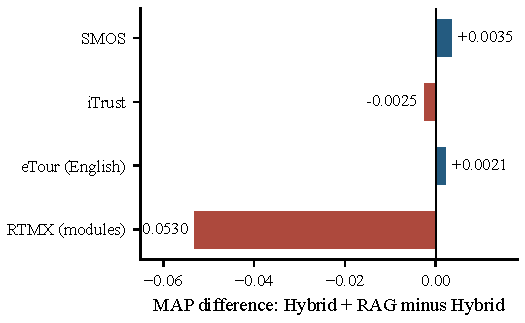
\includegraphics[width=\columnwidth]{figures/rag-delta.pdf}
\caption{Absolute MAP differences produced by top-five RAG reranking. Positive values favor reranking; negative values favor the hybrid baseline. No confidence intervals were estimated.}
\label{fig:delta}
\end{figure}

RAG reranking produces small MAP increases on SMOS (+0.0035) and eTour (+0.0021), alongside decreases on iTrust ($-0.0025$) and RTMX ($-0.0530$), as shown in Fig.~\ref{fig:delta}. Rankings change for 17/67, 60/105, 33/57, and 19/22 queries, respectively. Thus, frequent changes do not imply improved ranking. All 251 responses pass the recorded full-schema checks, yet this structural success coexists with lower retrieval effectiveness on two datasets. Semantic entailment and hallucination rates were not independently annotated.

As expected from the reranking rule, Recall@5 and Recall@10 remain unchanged. RTMX Recall@10 equals one for every method because its seven targets all fit within that cutoff. This ceiling makes MAP and early-rank behavior more informative than top-ten recall there. Likewise, eTour's graph-assisted MAP improvement does not imply improvement in every metric: micro top-ten precision, recall, and F1 change from 0.2930, 0.5422, and 0.3804 under hybrid retrieval to 0.2860, 0.5292, and 0.3713 with the graph. The learned ranker is rejected: validation MAP is 0.3051, below BM25's 0.3787.

\subsection{Consistency and Change Investigation}
All five consistency configurations return \texttt{UNCERTAIN} for every case. Each therefore agrees with 3/12 authored labels (25\%), exactly matching an always-uncertain baseline. The 60-call study provides no evidence of improved consistency classification. Five responses fail citation validation and remain uncertain; excluding them would conceal a reliability limitation. Schema/citation validity across the five configurations is 12/12, 11/12, 11/12, 11/12, and 10/12.

Recorded known-endpoint recall increases across configurations from 0 to 0, 0.20, 0.32, and 0.72. This indicates improved coverage of the partial authored endpoint sets in the richer configurations, not independently verified impact accuracy. In particular, temporal evidence and rule hypotheses are introduced together. Their individual effects cannot be separated. The broader controlled change records also retain a consumer-change miss involving four known endpoints, contradicting any perfect-impact claim.

The end-to-end example changes an API route from \texttt{/items} to \texttt{/catalog} while a client retains the old route. The saved run completes 12 tool stages, identifies 11 changed artifact records and 33 impact candidates, and verifies 24 source excerpts. Fifteen rule findings comprise ten lost-endpoint and five obsolete-consumer findings associated with the shared route change; they are not 15 independently confirmed defects. The model again returns uncertain. Total recorded duration is 33.65 seconds, including 25.10 seconds for the model stage. Mean generation durations for the four reranking datasets range from 37.93 to 70.82 seconds per query; these are observations under the saved CPU runs, not a controlled throughput benchmark.

\section{Discussion}
RQ1 has a project-dependent answer: lexical baselines remain competitive, graph relevance changes ranking trade-offs, and a schema-constrained small LLM can worsen an already retrieved ordering. Candidate truncation, limited context, and the supported-first policy are plausible contributors, but the experiments do not distinguish their causal effects. The results support retaining transparent baselines and examining rank changes rather than adopting RAG because its outputs are well formed.

For RQ2, richer evidence improves a partial coverage measure without improving label agreement. Evidence collection and decision making are distinct bottlenecks. An uncertain answer can be a defensible interface behavior when evidence is insufficient, but universal abstention is inadequate as an automatic consistency detector. Calibration and selective prediction would require independent labels and an explicit accuracy--coverage analysis that is not available here.

For RQ3, the recorded investigation demonstrates integration: revision differences, graph neighborhoods, exact quotes, rule hypotheses, and model uncertainty remain inspectable together. This supports developer review and reproducibility, but not an assurance guarantee. Compared with RAG traceability studies \cite{lissa,reqrag,ensemble}, the present study emphasizes this separation of evidence handling from semantic correctness. A local model avoids per-call commercial API charges; hardware, execution time, and maintenance still have costs. The unevaluated OmniRoute extension cannot be used to claim a stronger or universally free model configuration.

\section{Limitations and Threats to Validity}
\textit{Construct validity.} Ranking quality is not requirements conformance. Source-quote verification establishes provenance, not entailment; schema validity establishes output structure, not truth. Authored consistency labels and incomplete endpoint sets limit the meaning of agreement and coverage. The benchmark excludes unlinked queries, so its results cannot characterize false-positive behavior for requirements with no implementation.

\textit{Internal and conclusion validity.} There is one saved configuration per method, no independent semantic annotation, and no significance analysis. Exploratory graph weights and prompt choices may affect outcomes. The consistency configurations change several factors together, preventing an isolated attribution to graph use, agents, or temporal evidence. Reported latency includes differing contexts and resumable execution conditions. Audit agreement confirms arithmetic and record provenance, not the correctness of benchmark labels.

\textit{External validity.} Three Java retrieval datasets and a small Python module subset do not represent industrial polyglot systems. Controlled mutations are not independently discovered production defects. Static parsing misses dynamic behavior, chunk and prompt caps discard content, and the small local model is only one point in the quality--resource trade-off. The watcher has not been evaluated longitudinally; durable distributed execution and live OmniRoute accuracy remain unvalidated. These limits preclude claims of universal continuous assurance or general model superiority.

\section{Conclusion and Future Work}
Vigilant implements version-aware extraction, structural graphs, hybrid retrieval, checked evidence, and bounded agent orchestration for investigating relationships among requirements, code, and tests. Across 251 linked queries, local RAG reranking yields mixed MAP changes; the 60-call consistency study remains entirely uncertain and matches a 25\% always-uncertain baseline. A complete investigation demonstrates traceable evidence collection, while retaining uncertainty about semantic correctness. Future work should obtain independent artifact and consistency annotations, include no-link queries, isolate component effects, evaluate multiple model and prompt configurations under fixed budgets, and measure longitudinal behavior on real repository changes. The present evidence supports an auditable review framework and a reproducible evaluation, not an automatic correctness guarantee.
\balance
\begin{thebibliography}{14}
\bibitem{slr} N. Alturayeif, J. Hassine, and I. Ahmad, ``Machine learning approaches for automated software traceability: A systematic literature review,'' \emph{J. Syst. Softw.}, vol. 230, Art. no. 112536, 2025, doi: 10.1016/j.jss.2025.112536.
\bibitem{rag} P. Lewis \emph{et al.}, ``Retrieval-augmented generation for knowledge-intensive NLP tasks,'' in \emph{Adv. Neural Inf. Process. Syst.}, vol. 33, 2020, pp. 9459--9474.
\bibitem{lissa} D. Fuch\ss{} \emph{et al.}, ``LiSSA: Toward generic traceability link recovery through retrieval-augmented generation,'' in \emph{Proc. ICSE}, 2025, pp. 1396--1408, doi: 10.1109/ICSE55347.2025.00186.
\bibitem{bm25} S. Robertson and H. Zaragoza, ``The probabilistic relevance framework: BM25 and beyond,'' \emph{Found. Trends Inf. Retr.}, 2009, doi: 10.1561/1500000019.
\bibitem{sbert} N. Reimers and I. Gurevych, ``Sentence-BERT: Sentence embeddings using Siamese BERT-networks,'' in \emph{Proc. EMNLP-IJCNLP}, 2019, pp. 3982--3992, doi: 10.18653/v1/D19-1410.
\bibitem{reqrag} T. Hey, D. Fuch\ss{}, J. Keim, and A. Koziolek, ``Requirements traceability link recovery via retrieval-augmented generation,'' in \emph{Proc. REFSQ}, LNCS 15588, 2025, pp. 381--397, doi: 10.1007/978-3-031-88531-0\_27.
\bibitem{ensemble} D. Fuch\ss{}, S. Schwedt, J. Keim, and T. Hey, ``Beyond retrieval: A study of using LLM ensembles for candidate filtering in requirements traceability,'' in \emph{Proc. IEEE REW}, 2025, pp. 5--12, doi: 10.1109/REW66121.2025.00006.
\bibitem{archcons} J. Keim, S. Corallo, D. Fuch\ss{}, and A. Koziolek, ``Detecting inconsistencies in software architecture documentation using traceability link recovery,'' in \emph{Proc. ICSA}, 2023, pp. 141--152, doi: 10.1109/ICSA56044.2023.00021.
\bibitem{transarc} J. Keim, S. Corallo, D. Fuch\ss{}, T. Hey, T. Telge, and A. Koziolek, ``Recovering trace links between software documentation and code,'' in \emph{Proc. ICSE}, 2024, Art. no. 215, doi: 10.1145/3597503.3639130.
\bibitem{sweagent} J. Yang \emph{et al.}, ``SWE-agent: Agent-computer interfaces enable automated software engineering,'' arXiv:2405.15793, 2024.
\bibitem{minilm} Sentence Transformers, ``all-MiniLM-L6-v2,'' model card, revision 1110a243fdf4. [Online]. Available: \url{https://huggingface.co/sentence-transformers/all-MiniLM-L6-v2}
\bibitem{rrf} G. V. Cormack, C. L. A. Clarke, and S. Buettcher, ``Reciprocal rank fusion outperforms Condorcet and individual rank learning methods,'' in \emph{Proc. SIGIR}, 2009, pp. 758--759, doi: 10.1145/1571941.1572114.
\bibitem{qwen} Qwen Team, ``Qwen2.5-1.5B-Instruct,'' model card, revision 989aa7980e4c. [Online]. Available: \url{https://huggingface.co/Qwen/Qwen2.5-1.5B-Instruct}
\bibitem{rtmx} RTMX AI, ``rtmx-bench,'' source repository, commit c2ced5349577. [Online]. Available: \url{https://github.com/rtmx-ai/rtmx-bench}
\end{thebibliography}
\end{document}
